\documentclass[a4paper,14pt]{extarticle}
\usepackage[utf8]{inputenc}
\usepackage[russian]{babel}
\usepackage{amsmath,amsfonts,amssymb}
\usepackage{geometry}
\usepackage{graphicx}
\usepackage{url}
\usepackage[nottoc, notlof, notlot]{tocbibind}
\usepackage{listings}


\sloppy % Включаем "слабое" форматирование

\geometry{top=2cm, bottom=2cm, left=3cm, right=1.5cm}
\lstset{
    inputencoding=utf8,
    extendedchars=\true,
    literate={-}{{-}}1 {\->}{{\texttt{->}}}2 {_}{{\_}}1,
    basicstyle=\ttfamily,
    frame=single,
    captionpos=b,
}

\begin{document}

\begin{titlepage}
    \begin{center}
        Санкт-Петербургский политехнический университет Петра Великого\\
        Физико-механический институт\\[4cm]
        
        \textbf{Отчёт по лабораторной работе}\\[0.5cm]
        по дисциплине «Компьютерные сети»\\[0.5cm]
        \textbf{«Симуляция сети»}\\[4cm]
        
        \begin{flushleft}
            Выполнил\\
            студент гр. 5040102/30201 \hfill Завьялов И.В. \hfill \rule{3cm}{0.1pt} \\[1.5cm]
            Проверил\\
            доцент, к.ф.-м.н. \hfill \hspace{1.5cm} Баженов А.Н. \hfill \rule{3cm}{0.1pt} \\[1.5cm]
        \end{flushleft}
        
        \vfill
        Санкт-Петербург\\
        2024
    \end{center}
\end{titlepage}

\newpage

\tableofcontents

\newpage
\section{Постановка задачи}

Целью данной работы является моделирование и визуализация передачи пакетов по сети с использованием протоколов Go-Back-N (GBN) и Selective Repeat (SRP). В сети присутствуют промежуточные узлы (роутеры) с вероятностью отказа, в результате чего топология сети может изменяться в процессе передачи (изменение расположения удаляемых/добавляемых узлов). Это обуславливает динамическую перестройку маршрутов, необходимую для продолжения передачи пакетов между отправителем $A$ и получателем $B$.


\section{Теория}

\subsection{Протоколы GBN и SRP}
\textbf{Go-Back-N (GBN).} Данный протокол использует скользящее окно фиксированного размера. Отправитель последовательно отсылает пакеты, нумеруя их. Если в окно помещается $k$ пакетов, то отправитель может отослать эти $k$ пакетов подряд, не дожидаясь подтверждения каждого из них. При обнаружении утери хотя бы одного пакета, происходит откат — повторная передача с проблемного пакета и всех следующих.

\textbf{Selective Repeat (SRP).} В отличие от GBN, отправитель осуществляет переотправку только тех пакетов, которые были фактически утеряны или не получили подтверждения. Для этого приёмник хранит и может буферизовать некоторые пакеты вне очереди, а отправитель ведёт учёт подтверждений по каждому пакету в окне.

\subsection{Вероятность потери узлов и перестройка топологии}
В работе учитывается вероятность отказа промежуточных узлов, которая реализована путём случайного удаления узлов из сети через заданные интервалы времени. После удаления узлов производится добавление новых, чтобы общее количество активных роутеров оставалось неизменным. Для поиска маршрутов (кратчайшего пути по числу узлов или по геометрическому расстоянию) используется классический алгоритм Дейкстры (упрощённая модель OSPF).

\section{Реализация}

\textbf{Общая структура кода}

Код написан на языке Python с использованием библиотеки Pygame для визуализации. Основные составляющие модуля:
\begin{itemize}
    \item Реализация протоколов:
    \begin{itemize}
        \item Функции для отправителя/получателя GBN (\texttt{GBN\_sender}, \texttt{GBN\_receiver}).
        \item Функции для отправителя/получателя SRP (\texttt{SRP\_sender}, \texttt{SRP\_receiver}).
        \item Класс \texttt{Streaming}, объединяющий в себе состояние и логику отправителя/получателя для текущего протокола.
    \end{itemize}
    \item Алгоритм поиска пути: упрощённая реализация OSPF на базе алгоритма Дейкстры (\texttt{dijkstra()}), учитывающая евклидово расстояние между координатами узлов.
    \item Основной класс \texttt{NetworkSim}, который:
    \begin{itemize}
        \item Создаёт и хранит узлы сети ($A$, $B$ и заданное число промежуточных).
        \item Генерирует/обновляет топологию: определяет, какие узлы связаны на основе радиуса видимости (пороговое расстояние).
        \item Организует удаление/добавление узлов в соответствии с вероятностью отказа.
        \item Запускает или перезапускает передачу пакетов (стрим) при смене топологии или завершении передачи.
    \end{itemize}
    \item Функции визуализации (отрисовка узлов, рёбер, текучего “зелёного” прогресса по пути и т.д.).
\end{itemize}


\section{Результаты}
Скриншот примера работы программы представлен на рисунке 1.
\clearpage
\begin{figure}[htbp]
    \centering
    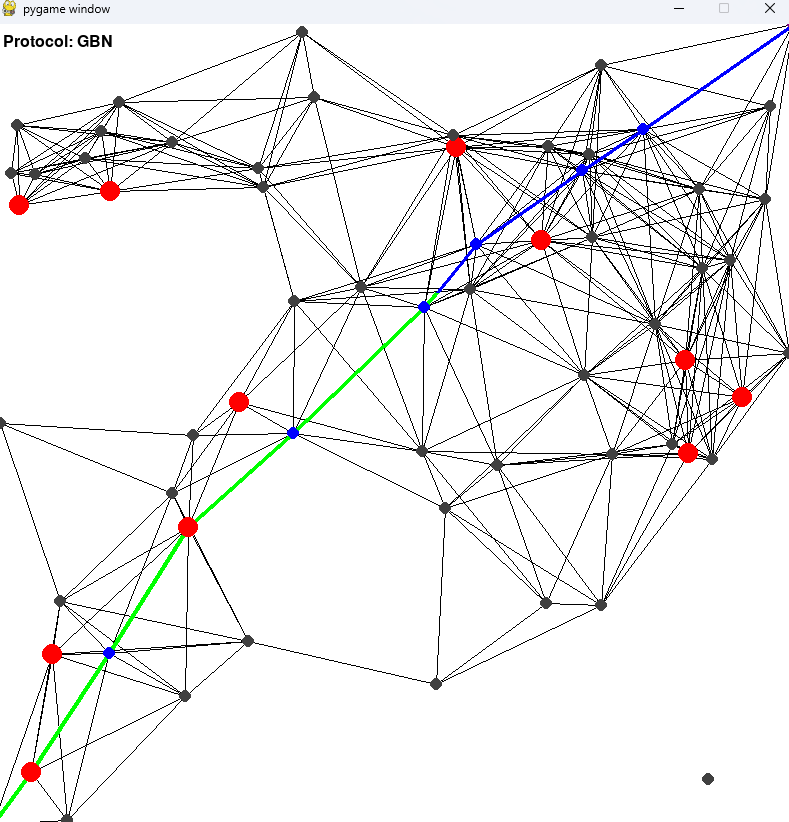
\includegraphics[width=0.8\textwidth]{im1.png}
    \caption{Скриншот примера работы программы}
    \label{fig:hamiltonianGraph}
\end{figure}

В результате выполнения работы получена модель сети, в которой:
\begin{itemize}
    \item Передача пакетов с использованием протоколов GBN или SRP наглядно демонстрируется на экране. При этом пользователь может визуально наблюдать:
    \begin{itemize}
        \item Топологию сети и как она изменяется со временем (появление/исчезновение узлов).
        \item Успешность или неуспешность доставки отдельных пакетов.
    \end{itemize}
    \item Перестройка топологии при отказах узлов влияет на то, может ли сеть обеспечить доставку. Когда узлы удаляются, и путь временно отсутствует, передача “подвисает”. Как только в сети снова появляется работающий маршрут, пакеты постепенно начинают доходить до получателя.
\end{itemize}


\section{Код и ресурсы}
Код проекта доступен в публичном репозитории на GitHub.

https://github.com/IlyaZawyalow/networks/tree/main/Lab3

\end{document}